
%%%%%%%%%%%%%%%%%%%%%%% file typeinst.tex %%%%%%%%%%%%%%%%%%%%%%%%%%%%%%
%
% This is the LaTeX source for the instructions to authors using
% the LaTeX document class SVMultln with class option 'lnicst'
% for contributions to the Lecture Notes of the Institute for
% Computer Sciences, Social-Informatics and
% Telecommunications Engineering series.
% www.springer.com/series/XXXX       Springer Heidelberg 2007/08/05
%
% It may be used as a template for your own input - copy it
% to a new file with a new name and use it as the basis for
% your article. It contains a few tweaked sections to demonstrate
% features of the package, though.
%
% If you have not much experiences with Springer LaTeX support,
% you should better use the special demonstration file "lnicst.tex"
% included in the LaTeX package for LNICST as template.
%
%%%%%%%%%%%%%%%%%%%%%%%%%%%%%%%%%%%%%%%%%%%%%%%%%%%%%%%%%%%%%%%%%%%%%%%%

\documentclass[lnicst,sechang,a4paper]{svmultln}
\usepackage{amssymb}
\setcounter{tocdepth}{3}
\usepackage{graphicx}

\usepackage{url}
\urldef{\mailsa}\path|{mohsin.khan, valtteri.niemi}@helsinki.fi|
\usepackage[pdfpagelabels,hypertexnames=false,breaklinks=true,bookmarksopen=true,bookmarksopenlevel=2]{hyperref}


%added by the author himself
\usepackage{color}
\usepackage[numbers]{natbib}
\usepackage{calc}
\usepackage{siunitx}
\DeclareSIUnit\mt{\milli\tesla} %% A method for say short cut or new unit!
\sisetup{inter-unit-product = {-}}

\begin{document}

\mainmatter  % start of an individual contribution

% first the title is needed
\title{Concealing IMSI in 5G Network Using Identity Based Crypto}

% a short form should be given in case it is too long for the running head
\titlerunning{Concealing IMSI in 5G Network Using Identity Based Crypto}

% the name(s) of the author(s) follow(s) next
%
% NB: Chinese authors should write their first names(s) in front of
% their surnames. This ensures that the names appear correctly in
% the running heads and the author index.
%
\author{Mohsin Khan%
%%\thanks{Please note that the LNICST Editorial assumes that all authors have used
%%the western naming convention, with given names preceding surnames. This determines
%%the structure of the names in the running heads and the author index.}%
\and Valtteri Niemi}  %
%\authorrunning{Lecture Notes of ICST: Authors' Instructions}
% (feature abused for this document to repeat the title also on left hand pages)

% the affiliations are given next
\institute{University of Helsinki, Department of Computer Science,\\
P.O. Box 68 (Gustaf H\"allstr\"amin katu 2b)\\
FI-00014 University of Helsinki\\
Finland\\
\mailsa
%\\
%\url{http://www.springer.com/series/7911}
}

%
% NB: a more complex sample for affiliations and the mapping to the
% corresponding authors can be found in the file "lnicst.dem",
% that is contained in the LNICST LaTeX support package.
%

\toctitle{AES and SNOW 3G are Feasible Choices}
\tocauthor{Authors' Instructions}
\maketitle


\begin{abstract}
The aspirations for the next generation mobile network (5G) are high. It has a vision of improved security and privacy over the existing LTE network. Subscription privacy of a user has been a historical concern with all the previous generation mobile networks, namely GSM, UMTS, and LTE. While a little improvements have been achieved in securing the privacy of long-term identity of a subscriber, the so called IMSI catchers are still in existence even in the LTE and advanced LTE networks. This report looks into this problem of concealing long-term identity of a subscriber and presents different techniques of using public-key cryptography to tackle it. One special case of public-key crytography is identity based crypto. A rigorous comparison among the pros and cons of the different techniques show that identity based crypto is a potential solution for securing the long-term identity privacy of a user in the 5G network.
\end{abstract}


\section{Introduction}
\label{intro} NGMN Alliance has pointed out the privacy of a user as a requirement of the 5G network under the requirement category of enhanced services \cite{NGMN_white_paper}. In 3GPP TR 33.899 \cite{TR33899}, subscribers' privacy is captured as one of the high level security requirements of the 5G network. However, in the context of diversified devices and complex business and service model of 5G, it is important to define who is a subscriber and what subscriber-privacy means. According to 3GPP TR 21.905 \cite{TR21905} a subscriber is an entity (associated with one or more users) that is engaged in a subscription with a service provider. A subscription describes the commercial relationship between the subscriber and the service provider, cf. 3GPP TR 21.905 \cite{TR21905}. A subscription identifier is the identifier that uniquely identifies a subscription in the 3GPP system. The identifier is used to access networks based on 3GPP specifications. Subscription Privacy refers to the right to the protection to any information that (a) can be used to identify a subscription to whom such information relates, or (b) is or might be directly or indirectly linked to a subscription. This definition of privacy suggests to protect any personally identifiable information (PII) from an active or passive attacker. While it is important to classify the identifiers into PII and non PII, the long-term identifier is surely a PII. in this report we will keep our discussion limited only to the case of long-term identifier of a subscriber. In the case of 2G, 3G and 4G networks, this long-term identifier is known as IMSI (International Mobile Subscriber Identity). Nevertheless, the same principles used in the solutions proposed in this report can be extended to conceal any PII.


One approach of protecting IMSI privacy is to use temporary IMSI instead of the original IMSI and keep changing the temporary IMSI at a feasible frequency. Note that the temporary IMSI has to be assigned over a confidentiality protected channel and different entities of the network may assign different temporary IMSIs to the user equipment (UE). In LTE network, the temporary IMSI assigned by serving network (SN) is called GUTI (Globally Unique Temporary ID) and the home network (HN) does not assign any temporary IMSI to the UE. However, during the initial attachment of a UE to the SN, the UE has neither a GUTI nor a security context with the SN that can assign it with a GUTI. Besides, GUTI can be lost either or both by the UE and the SN. This forces the UE to reveal its IMSI to the SN to keep itself from permanently locked out of the network. This problem gives an opportunity to an active IMSI catcher (AICa) who impersonates as a legitimate SN and force the UE to run the initial attachment protocol. This also gives an opportunity to a passive IMSI catcher (PICa) to eavesdrop the IMSI sent in clear text. Solutions \cite{pseudonym_valtteri_philip, pseudonym_ericsson} have been proposed by using temporary IMSI known as pseudonym assigned by the HN. While these solutions solve the cases of lost and unsynchronised GUTI, they still have the problem of lost or unsynchronised pseudonyms and also initial attachment. In this report we present how a security context can be set up in between the network (either with SN or HN) and the UE even before the identification of the UE so that the UE can use the security context to send its IMSI with confidentiality protection. Such a security context will mitigate the attack mounted by a PICa. Nevertheless, we show that an AICa would not be able to agree on a legitimate security context with the UE and consequently will not be able to reveal the IMSI.

\begin{figure}
\begin{center}
% Use the relevant command to insert your figure file.
% For example, with the graphicx package use
  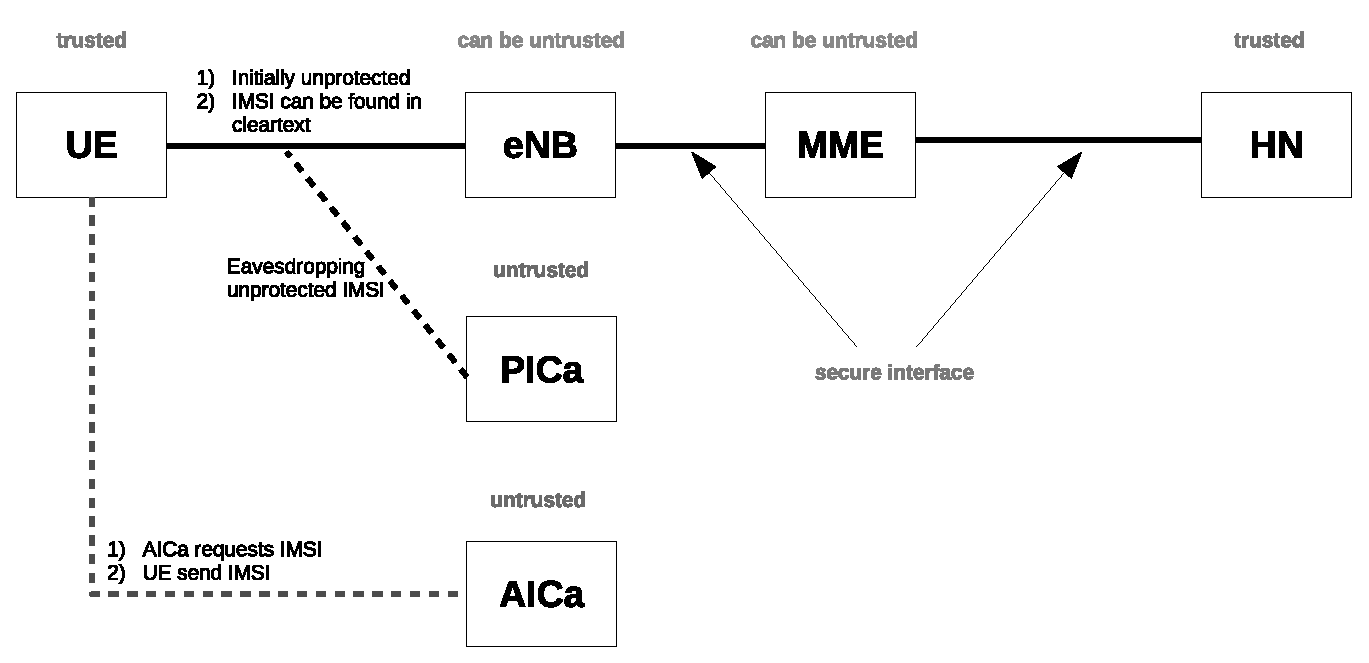
\includegraphics[width=.98\textwidth]{security_architecture_abstraction.eps}
% figure caption is below the figure
\caption{High-level security architecture}
\label{fig:security_architecture_abstraction}       % Give a unique label
\end{center}
\end{figure}

In order to present a formal discussion we need to know what are the entities involved in this identification process, what are the communication interfaces among those entities and how much the entities can be trusted with the IMSI.  As the architecture of 5G security is yet to be finalized, we present an abstraction of the involved entities and assume that whatever the security architecture of 5G eventually be, it will contain these entities and interfaces. This abstraction is directly extracted from LTE security architecture and we use some LTE acronyms to present the entities for better understanding. Figure \ref{fig:security_architecture_abstraction} shows the entities. It involves the UE, serving radio network (eNB), serving core network (MME), HN. We have two more entities: PICa and AICa. The interface  UE-NB in between UE and eNB is initially unprotected. Nevertheless, eNB-MME and MME-HSS are always protected and the security of these interfaces is out of the scope of this report. The PICas eavesdrop on the UE-eNB interface when it is unprotected to extract and IMSI. The AICas impersonate a legitimate SN and run a legitimate protocol with the UE in order to reveal the IMSI. HN and UE both owns the IMSI and they are trusted with it. Both of PICa and AICa are untrusted while it is technically possible to not trust eNB and MME. However, by some other specification in 3GPP TS \textcolor{red}{xx.xxx} it is required to reveal IMSI to the MME to enable lawful interception (LI) without involving HN. 

We propose different solutions based on public-key cryptography which make the UE-eNB interface protected even during the initial attachment to fight against the PICa. Our solutions also stop the AICa from running a legitimate protocol successfully that could reveal the IMSI. However, there are other 5G requirements which our solutions should also achieve. Such requirements are: reduced signalling overhead, improved control plane latency, concealing all the parts of IMSI (MCC, MNC and MSIN). To avoid the downgrade attack, the solutions need to be backward compatible with the legacy networks. Also, in the case of public-key, the complexity involved in setting a PKI and revocation of a publick-key need to be considered with high importance. Considering all these requirements, we evaluate our solutions based on the following criteria:
\begin{enumerate}
\item Concealed from PICa, AICa, eNB, MME
\item Parts of the IMSI concealed
\item Signalling overhead
\item Latency
\item Backward compatibility
\item PKI complexity
\item Public-key revocation and re-provisioning 
\end{enumerate}
While the choice of the solution is dependent on how much want to achieve, hybrid solution using identity based public-key cryptography and pseudonyms appear to be a promising solution.

\section{Public key cryptography against IMSI catchers}
Here we use public key cryptography which may or may not be based on identity based crypto to secure the privacy of the long term identity of a mobile phone user called IMSI (International mobile subscriber identity). We discuss different techniques of using the public key cryptography:

\begin{enumerate}
\item Identity based crypto based on the identity of SN where the HN is the key generator
\item HN assigned public private key pair for each SN
\item HN owned public private key pair
\end{enumerate}

In the consequent sections we describe the aforementioned techniques in further detail.

\section{Based on Identity of Serving Network} In this technique the HN has a public and private key pair. Every phone knows the public key of the HN. Whenever a SN asks the phone to provide its IMSI, the phone computes the public key of the SN using the public key of the HN. Then the phone encrypts the IMSI with the computed public key of the SN and sends it to the SN along with the HN identity. The SN obtains (possibly already have obtained) its private key from the mentioned HN. Using this private key, the SN can decrypt IMSI. Figure \ref{fig:IBC} represents the high level protocol.

\subsection{Concerns and Solutions}
\begin{enumerate}
\item How to provision, revoke and re-provision the public key of HN in the phone?
\item How to black list a SN?
\end{enumerate}

\subsection{Based on HN generated public private key pair for every SN}

\section{Conclusion}
\label{sec:conclusion}

\section{Acknowledgement}
\label{sec:acknowledgement}



\begin{thebibliography}{4}

\bibitem{NGMN_white_paper} NGMN 5G White Paper V1.0 [cited Jan, 2017]. Available at: https://www.ngmn.org/uploads/media/NGMN\_5G\_White\_Paper\_V1\_0.pdf

\bibitem{TR33899} 3GPP TR 33.899 V0.6.0 [cited Jan, 2017]. Available at: https://portal.3gpp.org/desktopmodules/Specifications/SpecificationDetails.aspx?\\specificationId=3045

\bibitem{TR21905} 3GPP TR 21.905 [cited Jan, 2017]. Available at: https://portal.3gpp.org/desktopmodules/Specifications/SpecificationDetails.aspx?\\specificationId=558


\bibitem{pseudonym_ericsson} Karl Norrman, Mats Näslund, Elena Dubrova: Protecting IMSI and User Privacy in 5G Networks. 2nd International Workshop on 5G Security

\bibitem{pseudonym_valtteri_philip} Philip Ginzboorg,  Valtteri Niemi: Privacy of the long-term identities in cellular networks. Proceedings of the 9th EAI International Conference on Mobile Multimedia Communications
Pages 167-175




\end{thebibliography}

\end{document}
